\documentclass[
  captions=tableheading,
  bibliography=totoc, 
  titepage=firstiscover,
]{scrartcl}

\usepackage{blindtext} %neuer input

\usepackage{longtable} % Tabellen über mehrere Seiten

\usepackage[utf8]{inputenc} %neuer input

\usepackage{scrhack}

\usepackage[aux]{rerunfilecheck} %Warnung falls nochmal kompiliert werden muss

\usepackage{fontspec} %Fonteinstellungen

\recalctypearea{}

\usepackage[main=ngerman]{babel} %deutsche Spracheinstellung

\usepackage{ragged2e} %neuer input

\usepackage{amsmath, nccmath}

\usepackage{amssymb} %viele mathe Symbole

\usepackage{mathtools} %Erweiterungen für amsmath


\DeclarePairedDelimiter{\abs}{\lvert}{\rvert}
\DeclarePairedDelimiter{\norm}{\lVert}{\rVert}

\DeclarePairedDelimiter{\bra}{\langle}{\rvert}
\DeclarePairedDelimiter{\ket}{\lvert}{\rangle}

\DeclarePairedDelimiterX{\braket}[2]{\langle}{\rangle}{
#1 \delimsize| #2
}

\NewDocumentCommand \dif {m}
{
\mathinner{\symup{d} #1}
}


\usepackage[
  math-style=ISO,
  bold-style=ISO,
  sans-style=italic,
  nabla=upright,
  partial=upright,
  warnings-off={
    mathtools-colon,
    mathtools-overbracket,
  },
]{unicode-math}

\setmathfont{Latin Modern Math}
\setmathfont{XITS Math}[range={scr, bfscr}]
\setmathfont{XITS Math}[range={cal, bfcal}, StylisticSet=1]


\usepackage[
  locale=DE,
  separate-uncertainty=true,
  per-mode=reciprocal,
  output-decimal-marker={,},
]{siunitx}

\usepackage[autostyle]{csquotes} %richtige Anführungszeichen

\usepackage{xfrac}

\usepackage{float}

\floatplacement{figure}{htbp}

\floatplacement{table}{htbp}

\usepackage[ %floats innerhalb einer section halten
  section,   %floats innerhalb er section halten
  below,     %unterhalb der Section aber auf der selben Seite ist ok
]{placeins}

\usepackage[
  labelfont=bf,
  font=small,
  width=0.9\textwidth,
]{caption}

\usepackage{subcaption} %subfigure, subtable, subref

\usepackage{graphicx}

\usepackage{grffile}

\usepackage{booktabs}

\usepackage{microtype} %Verbesserungen am Schriftbild

\usepackage[
backend=biber,
]{biblatex}

\addbibresource{../lit.bib}

\usepackage[ %Hyperlinks im Dokument
  german,
  unicode,
  pdfusetitle,
  pdfcreator={},
  pdfproducer={},
]{hyperref}

\usepackage{bookmark}

\usepackage[shortcuts]{extdash}

%\usepackage{warpcol}


\begin{document}
    \title{V101 Das Trägheitsmoment}
    \author{  
    Tobias Rücker\\
    \texorpdfstring{\href{mailto:tobias.ruecker@tu-dortmund.de}{tobias.ruecker@tu-dortmund.de}
    \and}{,} 
    Paul Störbrock\\
    \texorpdfstring{\href{mailto:paul.stoerbrock@tu-dortmund.de}{paul.stoerbrock@tu-dortmund.de}}{}
    }
    \date{Durchführung: 03.12.2019, Abgabe: 10.12.2019\vspace{-4ex}}
\maketitle
\center{\Large Versuchsgruppe: \textbf{42}}
    
    \begin{abstract}
    \centering
        \textbf{Ziel:} Messung des Trägheitsmoments verschiedener Körper und Nachweis des Satzes von Steiner
    \end{abstract}

\newpage
\tableofcontents
\newpage

% Ziel %%%%%%%%%%%%%%%%%%%%%%%%%%%%%%%%%%%%%%%%%%%%%%%%%%%%%%%%%%%%%%%%%%%%%%%%%%%%%%%%%%%%%%%%%%%%%%%%%
\section{\textbf{Ziel}}

% Theorie %%%%%%%%%%%%%%%%%%%%%%%%%%%%%%%%%%%%%%%%%%%%%%%%%%%%%%%%%%%%%%%%%%%%%%%%%%%%%%%%%%%%%%%%%%%%%%%%%
\section{Theorie}\justifying
\begin{align}
    \intertext{Rotationsbewegungen beschreiben Bewegungen bei denen sich eine Massenverteilung
    um eine Rotationsachse dreht. Dabei werden diese Bewegungen hauptsächlich durch die Größen
    beschrieben: dem Trägheitsmoment $I$, dem Drehmoment $M$ und der Winkelbeschleunigung $\dot{\omega}$.
    Das Trägheitsmoment beschreibt dabei eine skalare Größe, welche ein Maß der Trägheit einer Massenverteilung
    gegenüber Rotationen darstellen. Es bildet damit ein Äquivalent zur Masse in Translationsbewegungen.
    Ein Trägheitsmoment hängt dabei explizit von dem Abstand zur und der Wahl der Rotationsachse ab.
    Für eine Punktmasse zum Beispiel, lässt sich das Trägheitsmoment durch folgende Formel 
    beschreiben \cite{V101}:
    }
    I &= m  r^2 \label{eq:1}
    \intertext{Für ausgedehnte Massekörper wird diese Formel über infinitesimal kleine Massestücke aufintegriert \cite{V101}:
    }
    I &= \int r^2 \symup{d} \, m \label{eq:2}
    \intertext{Für homogene Körper lassen sich diese Integrale einfach lösen. 
    Einige Beispiele für Trägheitsmomente einfacher Körper sind das Trägheitsmoment einer homogenen Vollkugel durch seinen 
    Mittelpunkt \cite{V101}:
    }
    I_{\text{Kugel}} &= \frac{2}{5} m R^2 \label{eq:3}
    \intertext{Das Trägheitsmoment eines homogenen Vollzylinders mit der Drehachse durch den  Mittelpunkt des Bodens \cite{V101}:
    }
    I_{\text{Zylinder,v}} &= \frac{mR^2}{2} \label{eq:4}
    \intertext{Und das Trägheitsmoment eines homogenen Vollzylinders deren Drehachse senkrecht zum Mantel durch den
    Schwerpunkt verläuft \cite{V101}:
    }
    I_{\text{Zylinder,h}} &= m \left( \frac{R^2}{4}+\frac{h^2}{12} \right) \label{eq:5}
    \intertext{Bei komplexeren Körper wird versucht den Schwerpunkt durch eine Zusammensetzung einfacher Körper zu beschreiben.
    Verläuft die Drehachse parallel zu einer Achse durch den Schwerpunkt, wird das Trägheitsmoment
    mithilfe des Steinerschen Satzes berechnet \cite{V101}:
    }
    I &= I_s+m \cdot a^2 \label{eq:6}
    \intertext{$I_s$ beschreibt dabei das Trägheitsmoment bezüglich der parallelen Drehachse durch den Schwerpunkt.
    Die skalare Größe $a$ stellt dabei den Abstand der beiden parallelen Achsen dar.
    Das Drehmoment ist definiert als die Kraft, welche an einen drehenden Körper ansetzt.
    Beschreiben lässt sich dieser durch \cite{V101}:
    }
    \vec{M} &= \vec{F} \times \vec{r} \label{eq:7}
    \intertext{Liegt nun ein oszillierendes System vor, welches um einen Winkel $\varphi$
    ausgelenkt wird, so wirkt der Feder eine rücktreibende Kraft der Bewegung entgegen.
    Die Periodendauer der Schwingung kann dabei beschrieben werden durch \cite{V101}:
    }
    T &= 2 \pi \sqrt{\frac{I}{D}} \label{eq:8}
    \intertext{Wobei das Dremoment $M$ und die Winkelrichtgröße $D$ in folgender Beziehung
    stehen \cite{V101}:
    }
    M &= D \cdot \varphi \label{eq:9}
\end{align}

% Fehlerrechnung %%%%%%%%%%%%%%%%%%%%%%%%%%%%%%%%%%%%%%%%%%%%%%%%%%%%%%%%%%%%%%%%%%%%%%%%%%%%%%%%%%%%%%%%%%%%%%%%%%%
\section{Fehlerrechnung}\justifying
Für die Auswertung werden im folgenden diese Formeln zur Bestimmung der Fehler verwendet:
\begin{subequations}
\begin{align}
\intertext{Der Mittelwert wird berechnet mit:
}
    \overline{x} &= \frac{1}{N}\sum_{i=1}^{N} x_i \label{eq:10a}.
\intertext{Der Fehler des Mittelwerts wird berechnet:
}
    \Delta\overline{x} &= \frac{1}{\sqrt{N}} \sqrt{\frac{1}{1-N} \sum_{i=1}^{N} (x_i - \overline{x})^2} \label{eq:10b},
\intertext{Und die Gaußsche Fehlerfortpflanzung wird mit der folgenden Formel berechnet:
}
    \Delta f &= \sqrt{\sum_{i=1}^{N} \left( \frac{\delta f}{\delta x_i} \right)^2 \cdot (\Delta x_i)^2} \label{eq:10c}
\intertext{Zur Berechnung von Ausgleichsgeraden werden dabei}
        y &= m \cdot x + b \label{eq:10d} \\ 
        m &= \frac{\overline{xy} - \overline{x} \cdot \overline{y}}{\overline{x^2} - {\overline{x}}^2} \label{eq:10e} \qquad \qquad\\
        b &= \frac{\overline{y} \cdot \overline{x^2} - \overline{xy} \cdot \overline{x}}{\overline{x^2} - {\overline{x}}^2} \label{eq:10f}
\end{align}
\end{subequations}


% Versuchsaufbau %%%%%%%%%%%%%%%%%%%%%%%%%%%%%%%%%%%%%%%%%%%%%%%%%%%%%%%%%%%%%%%%%%%%%%%%%%%%%%%%%%%%%%%%%%%%%%%%%%%%%%%%%%%%%%%%%%%%%%%%%%%%%%%%%%%%%%%%%%%
\section{Versuchsaufbau}\justifying

Benötigt werden: \textit{Eine Drehachse die durch eine Spiralfeder mit einem festen Rahmen verbunden ist, eine Stabachse der Länge $\SI{62}{\centi\meter}$, 
zwei identische zylindrische Gewichte ($\SI{261.5}{\gram}$), eine Kugel mit Aufsatz (m=$\SI{1168.5}{\gram}$, r=$\SI{7.3}{\centi\meter}$), einen Zylinder mit 
Aufsatz (m=$\SI{1525.5}{\gram}$, h=$\SI{13,95}{\centi\meter}$, d=$\SI{8}{\centi\meter}$), eine Holzpuppe mit Aufsatz ($\rho=\SI{780}{\kilo\gram\per\cubic\meter}$), 
ein Newtonmeter (von $\SI{0.1}{\newton}$ bis $\SI{1}{\newton}$), eine Drehwinkel-Messscheibe, ein Ma\ss band, eine Schieblehre, eine Stopuhr.}\\
Zu Beginn wird die Stabachse horizontal auf der Drehachse befestigt. An beiden Enden der Stabachse werden die beiden zylindrischen Gewichte angebracht.
Anschließend wird die Kugel auf die Drehachse gesteckt.
Der Zylinder wird längs auf der Drehachse aufgesteckt. 
Zum Schluss wird die Puppe in einer stehenden Position, einmal mit angelegten Armen und einmal mit ausgestreckten, senkrecht zum Körper befindlichen
Armen, auf der Drehachse befestigt.

% Versuchsdurchführung %%%%%%%%%%%%%%%%%%%%%%%%%%%%%%%%%%%%%%%%%%%%%%%%%%%%%%%%%%%%%%%%%%%%%%%%%%%%%%%%%%%%%%%%%%%%%%%%%%%%%%%%%%%%%%%%%%%%%%%%%%%%%%%%%%%%%%%%%%%
\section{Versuchsdurchführung}\justifying

Um die Trägheitsmomente der einzelnen Körper zu berechnen, soll zuerst das Trägheitsmoment der Drehachse bestimmt werden. Infolgedessen wird die
Stabachse auf der Drehachse befestigt. Die beiden zylindrischen Gewichte werden mit einem Abstand von $\SI{25}{\centi\meter}$ zur Mitte an beiden 
Enden der Stabachse angebracht. Daraufhin wird die Stabachse um einen konstanten Winkel $\varphi = \SI{20}{\degree}$ ausgelenkt und die Periodendauer mithilfe
einer Stoppuhr über drei Perioden genau zweimal gemessen. Dies wird für jede Reduzierung des Abstandes um $\SI{2.5}{\centi\meter}$ wiederholt, bis beide 
Massen bei einem Abstand von $\SI{2.5}{\centi\meter}$ zur Mitte angekommen sind.\\
Neben dem Trägheitsmoment der Drehachse ist die Federkonstante der Spiralfeder für die folgenden Trägheitsmomente wichtig. Um diese zu bestimmen 
werden die Massen von der Stabachse genommen und diese um einen Winkel von $\SI{90}{\degree}$  ausgelenkt. Nun wird das Newtonmeter an einem konstanten Abstand von 
$\SI{30}{\centi\meter}$ zur Mitte angesetzt und die Kraft der Spiralfeder übers Newtonmeter aufgenommen. Dabei wird das Newtonmeter
senkrecht zum Radius der Kreisbahn gehalten. Anschließend werden die Kräfte für eine schrittweise Erhöhung des Auslenkwinkels um $\SI{10}{\degree}$ gemessen,
bis der ein Wert von $\SI{260}{\degree}$ erreicht wird.\\
Nachdem Federkonstante und Trägheitsmoment der Drehachse bestimmt wurden, können die Trägheitsmomente des Zylinders, der Kugel und der Puppe
errechnet werden. Für die Kugel werden fünf Werte für die Schwingdauer einer Periode $T$ bei einem konstanten Winkel von $\SI{20}{\degree}$ erfasst.
Für den Zylinder werden ebenfalls fünf Messwerte für eine Periode aufgenommen, bei einem konstanten Winkel von $\SI{10}{\degree}$. 
Zuletzt werden die Schwingperioden der Puppe in Position 1 (Arme angelegt) und Position 2 (Arme ausgestreckt) gemessen. Dafür wurde der Auslenkwinkel
bei $\SI{10}{\degree}$ konstant gehalten. Um bei einer kurzen Schwingdauer verlässliche Messwerte zu erhalten, wurde die Zeitlupenfunktion einer 
Handykamera verwendet. Das Video zeigt die Schwingung der Puppe und die Stopuhr, welche den zeitlichen Verlauf der Schwingung verdeutlicht.\\

% Auswertung %%%%%%%%%%%%%%%%%%%%%%%%%%%%%%%%%%%%%%%%%%%%%%%%%%%%%%%%%%%%%%%%%%%%%%%%%%%%%%%%%%%%%%%%%%%%%%%%%%%%%%%%%%%%%%%%%%%%%%%%%%%%%%%%%%%%%%%%%%%
\section{Auswertung}\justifying

\subsection{Die Drehachse}\justifying % Drehachse ---------------------------------------------------------------------------------------------------------

\flushleft{Um\;}\justifying das Trägheitsmoment der Drehachse zu bestimmen wird die Formel \eqref{eq:8} nach I umgestellt und mit Formel % Trägheitsmoment I_D ---------------------------------------------------------------------------------------------------------
\eqref{eq:6} gleichgesetzt. Die resultierende Gleichung sieht aus wie folgt:
\begin{equation}
T^2 = I_S \cdot \frac{4\pi^2}{D} + \frac{m_k \cdot 4\pi^2}{D} \cdot a^2\label{eq:11}
\end{equation} 
Hierbei wird festgestellt, dass
\begin{align}
    b=I_S \cdot \frac{4\pi^2}{D} \label{eq:12}
\end{align}
entspricht.\\
Daraus folgt für das Trägheitsmoment der Drillachse:
\begin{align}
    I_D = \frac{b \cdot D}{4 \pi^2} \label{eq:13}
\end{align}

\begin{table}[H]
    \centering
    \input{table_IStab.tex}
    \caption{Tabelle der Messwerte für das Trägheitsmoment der Stabachse $I_D$}
    \label{tab:IStab}
\end{table}

\flushleft{Für} die Berechnung wurden zwei Werte der Periodendauer für einen Abstand gemessen und in der Tabelle \ref{tab:IStab}
zusammengetragen. Diese zwei Werte wurden gemittelt und auf eine Periode normiert.

\flushleft{Mithilfe\;}\justifying der Formel \eqref{eq:12} und dem Pyton Befehl linregress() \cite{numpy} lässt sich die Geradengleichung
des folgenden Graphen \ref{fig:1} bestimmen. 
\flushleft{Dabei\;}\justifying sehen die Steigung $m$ und der Schnittpunkt der y-Achse $b$ des Graphen \ref{fig:1} folgendermaßen aus:

\begin{subequations}
\begin{align}
m &= \text{\input{slope.tex}}\label{eq:14a}\\
b &= \text{\input{intercept.tex}}\label{eq:14b}
\end{align}
\end{subequations}
\newpage

\begin{figure}[H]
    \centering
    \includegraphics[width=\textwidth]{plot.pdf}
    \caption{Lineare Regression für $I_{Stab}$}
    \label{fig:1}
\end{figure}


\flushleft{Aus\;}\justifying der linearen Regression lässt sich das Trägheitsmoment der Drehachse mit Formel \eqref{eq:13} bestimmten:
\begin{equation}
I_D = \input{I_D.tex}\label{eq:15} % Trägheitsmoment Drehachse
\end{equation}

% Federkonstante --------------------------------------------------------------------------------------------------------------------------

\flushleft{Für\;}\justifying die Federkonstante wurde die Formel \eqref{eq:7} mit der Formel \eqref{eq:9} gleichgesetzt. Formel \eqref{eq:7} kann durch $M = \abs{\vec{F}} \cdot \abs{\vec{r}}$
dargestellt werden, da die Kraft der rücktreibenden Kraft senkrecht zum Radius steht. Wird die gewonnene Gleichung nach $D$ umgestellt, folgt:
\begin{equation}
D = \frac{F\cdot r}{\varphi}\label{eq:16}
\end{equation}

\begin{table}[H]
    \centering
    \input{table_D.tex}
    \caption{Tabelle der Messwerte für die Federkonstante $D$}
    \label{tab:D}
\end{table}


\flushleft{Die\;}\justifying Federkonstante der Spiralfeder berechnet sich aus dem Mittelwert \eqref{eq:10a} der einzelnen $D$'s aus 
Formel \eqref{eq:12} mit den Werten aus Tabelle \ref{tab:D} und ergibt:

\begin{equation}
\overline{D} = \text{\input{D_mean.tex}} \label{eq:17} % Federkonstante der Spiralfeder
\end{equation}

\subsection{Der Zylinder}\justifying % Zylinder ---------------------------------------------------------------------------------------------------------

\begin{table}[H]
    \centering
    \input{table_I.tex}
    \caption{Tabelle der Messwerte für die Perioden $T$ der einzelnen Körper}
    \label{tab:I}
\end{table}


\flushleft{Für\;}\justifying den errechneten Wert des Trägheitsmoments des Zylinders wurde die Formel \eqref{eq:11} nach $I_S$ umgestellt.
Die Werte für die Periodendauer aus der Tabelle \ref{tab:I} wurden auf für die folglenden Berechnungen auf eine Nachkommastelle gerundet.
Daraus folgt das errechnete Trägheitsmoment des Zylinders mit den Werten aus Tabelle \ref{tab:I} und einer Masse von $\SI{1525.5}{\gram}$:
\begin{equation}
I_{Zy, exp.} = \input{I_Zylinder_mean.tex}\label{eq:18}
\end{equation}

\flushleft{Das\;}\justifying theoretische Trägheitsmoment des Zylinders wurde mit der Formel \eqref{eq:5} und den Werten für $T$ aus Tabelle 
\ref{tab:I} bestimmt und lautet:
\begin{equation}
I_{Zy, lit.} = \input{I_Zylinder_Theorie.tex}\label{eq:19}
\end{equation}

\flushleft{Der\;}\justifying daraus resultierende relative Fehler des Trägheitsmoments vom Zylinder beträgt:
\begin{equation}
\frac{I_{Zy, exp.} - I_{Zy, lit.}}{I_{Zy, lit.}} = \input{RF_I_Zylinder.tex}\label{eq:20}
\end{equation}
\newpage

\subsection{Die Kugel}\justifying % Kugel ---------------------------------------------------------------------------------------------------------

\flushleft{Das\;}\justifying errechnete Trägheitsmoment der Kugel ist:
\input{I_Kugel_mean.tex}

\flushleft{Das\;}\justifying theoretische Trägheitsmoment der Kugel ist:
\input{I_Kugel_Theorie.tex}

\flushleft{Der\;}\justifying relative Fehler des Trägheitsmoments der Kugel ist:
\input{RF_I_Kugel.tex}

\subsection{Puppe (Position 1)}\justifying % Puppe 1 ---------------------------------------------------------------------------------------------------------

\begin{figure}[H]
\caption{Positionen der Puppe}
\begin{subfigure}{0.495\linewidth}
\centering
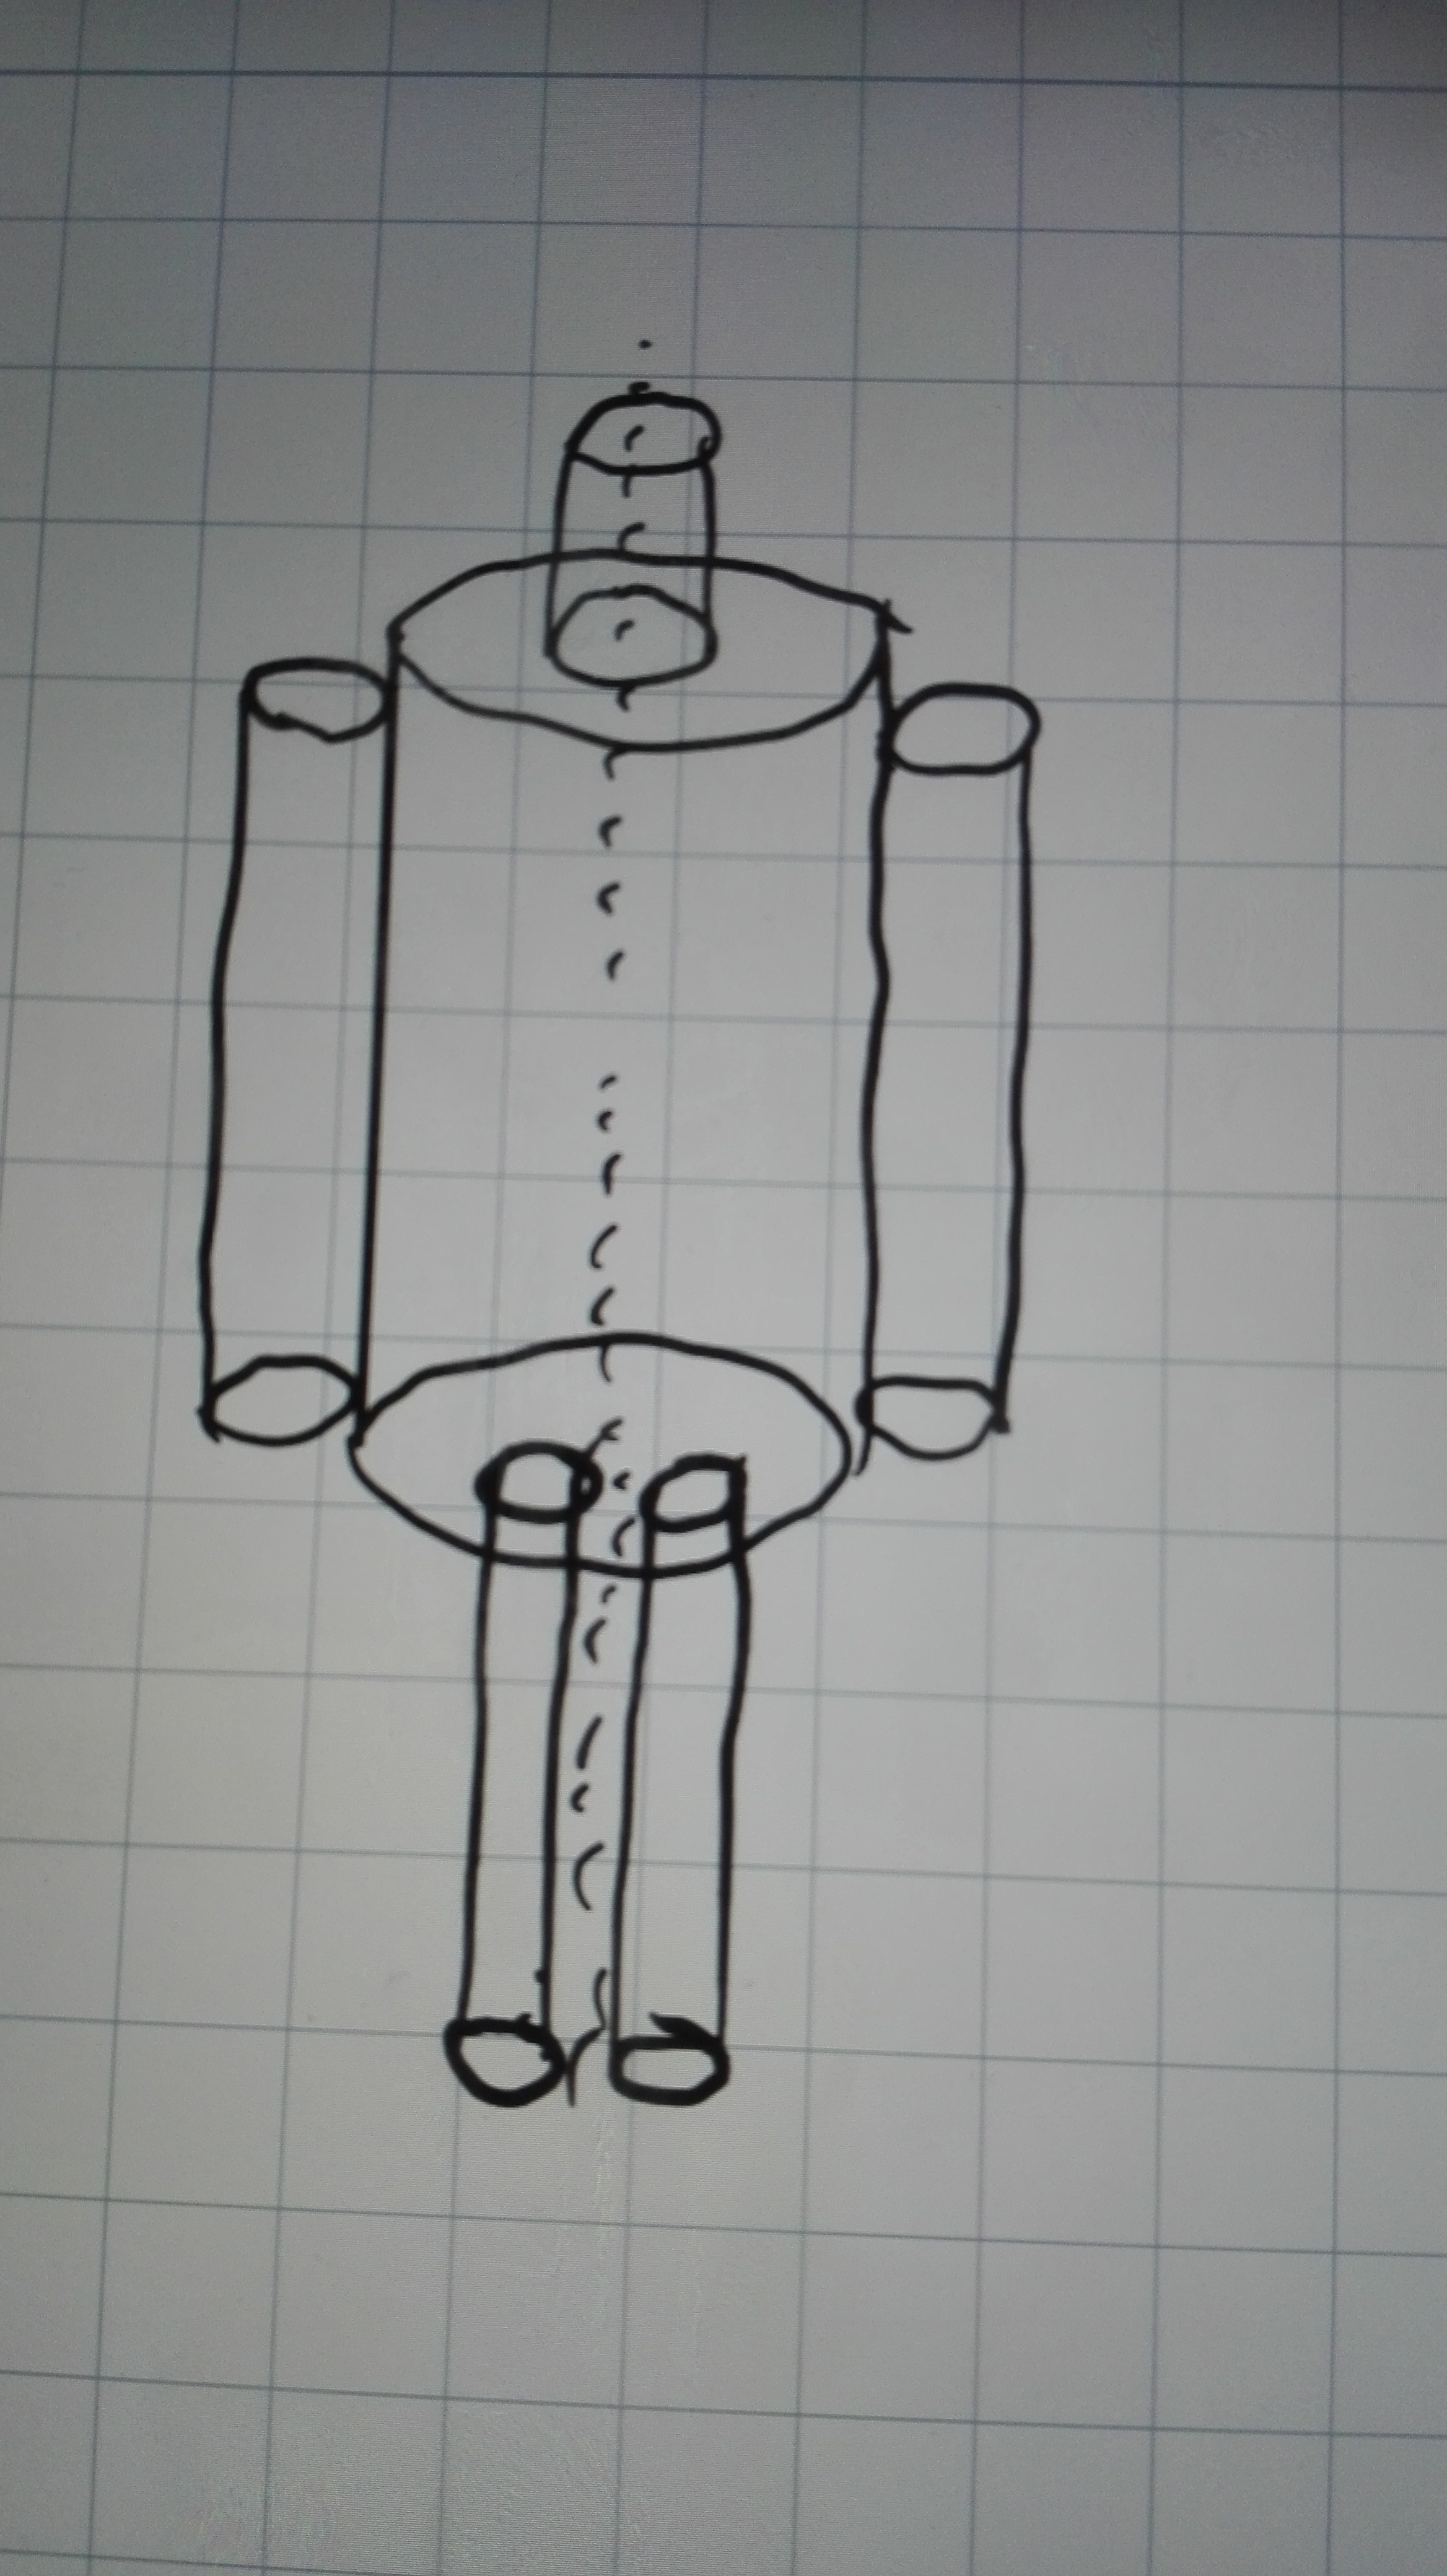
\includegraphics[width=\textwidth]{images/puppe_an.jpg}
\caption{Puppe mit angezogenen Armen (Pos. 1)}
\end{subfigure}
\begin{subfigure}{0.495\linewidth}
\centering
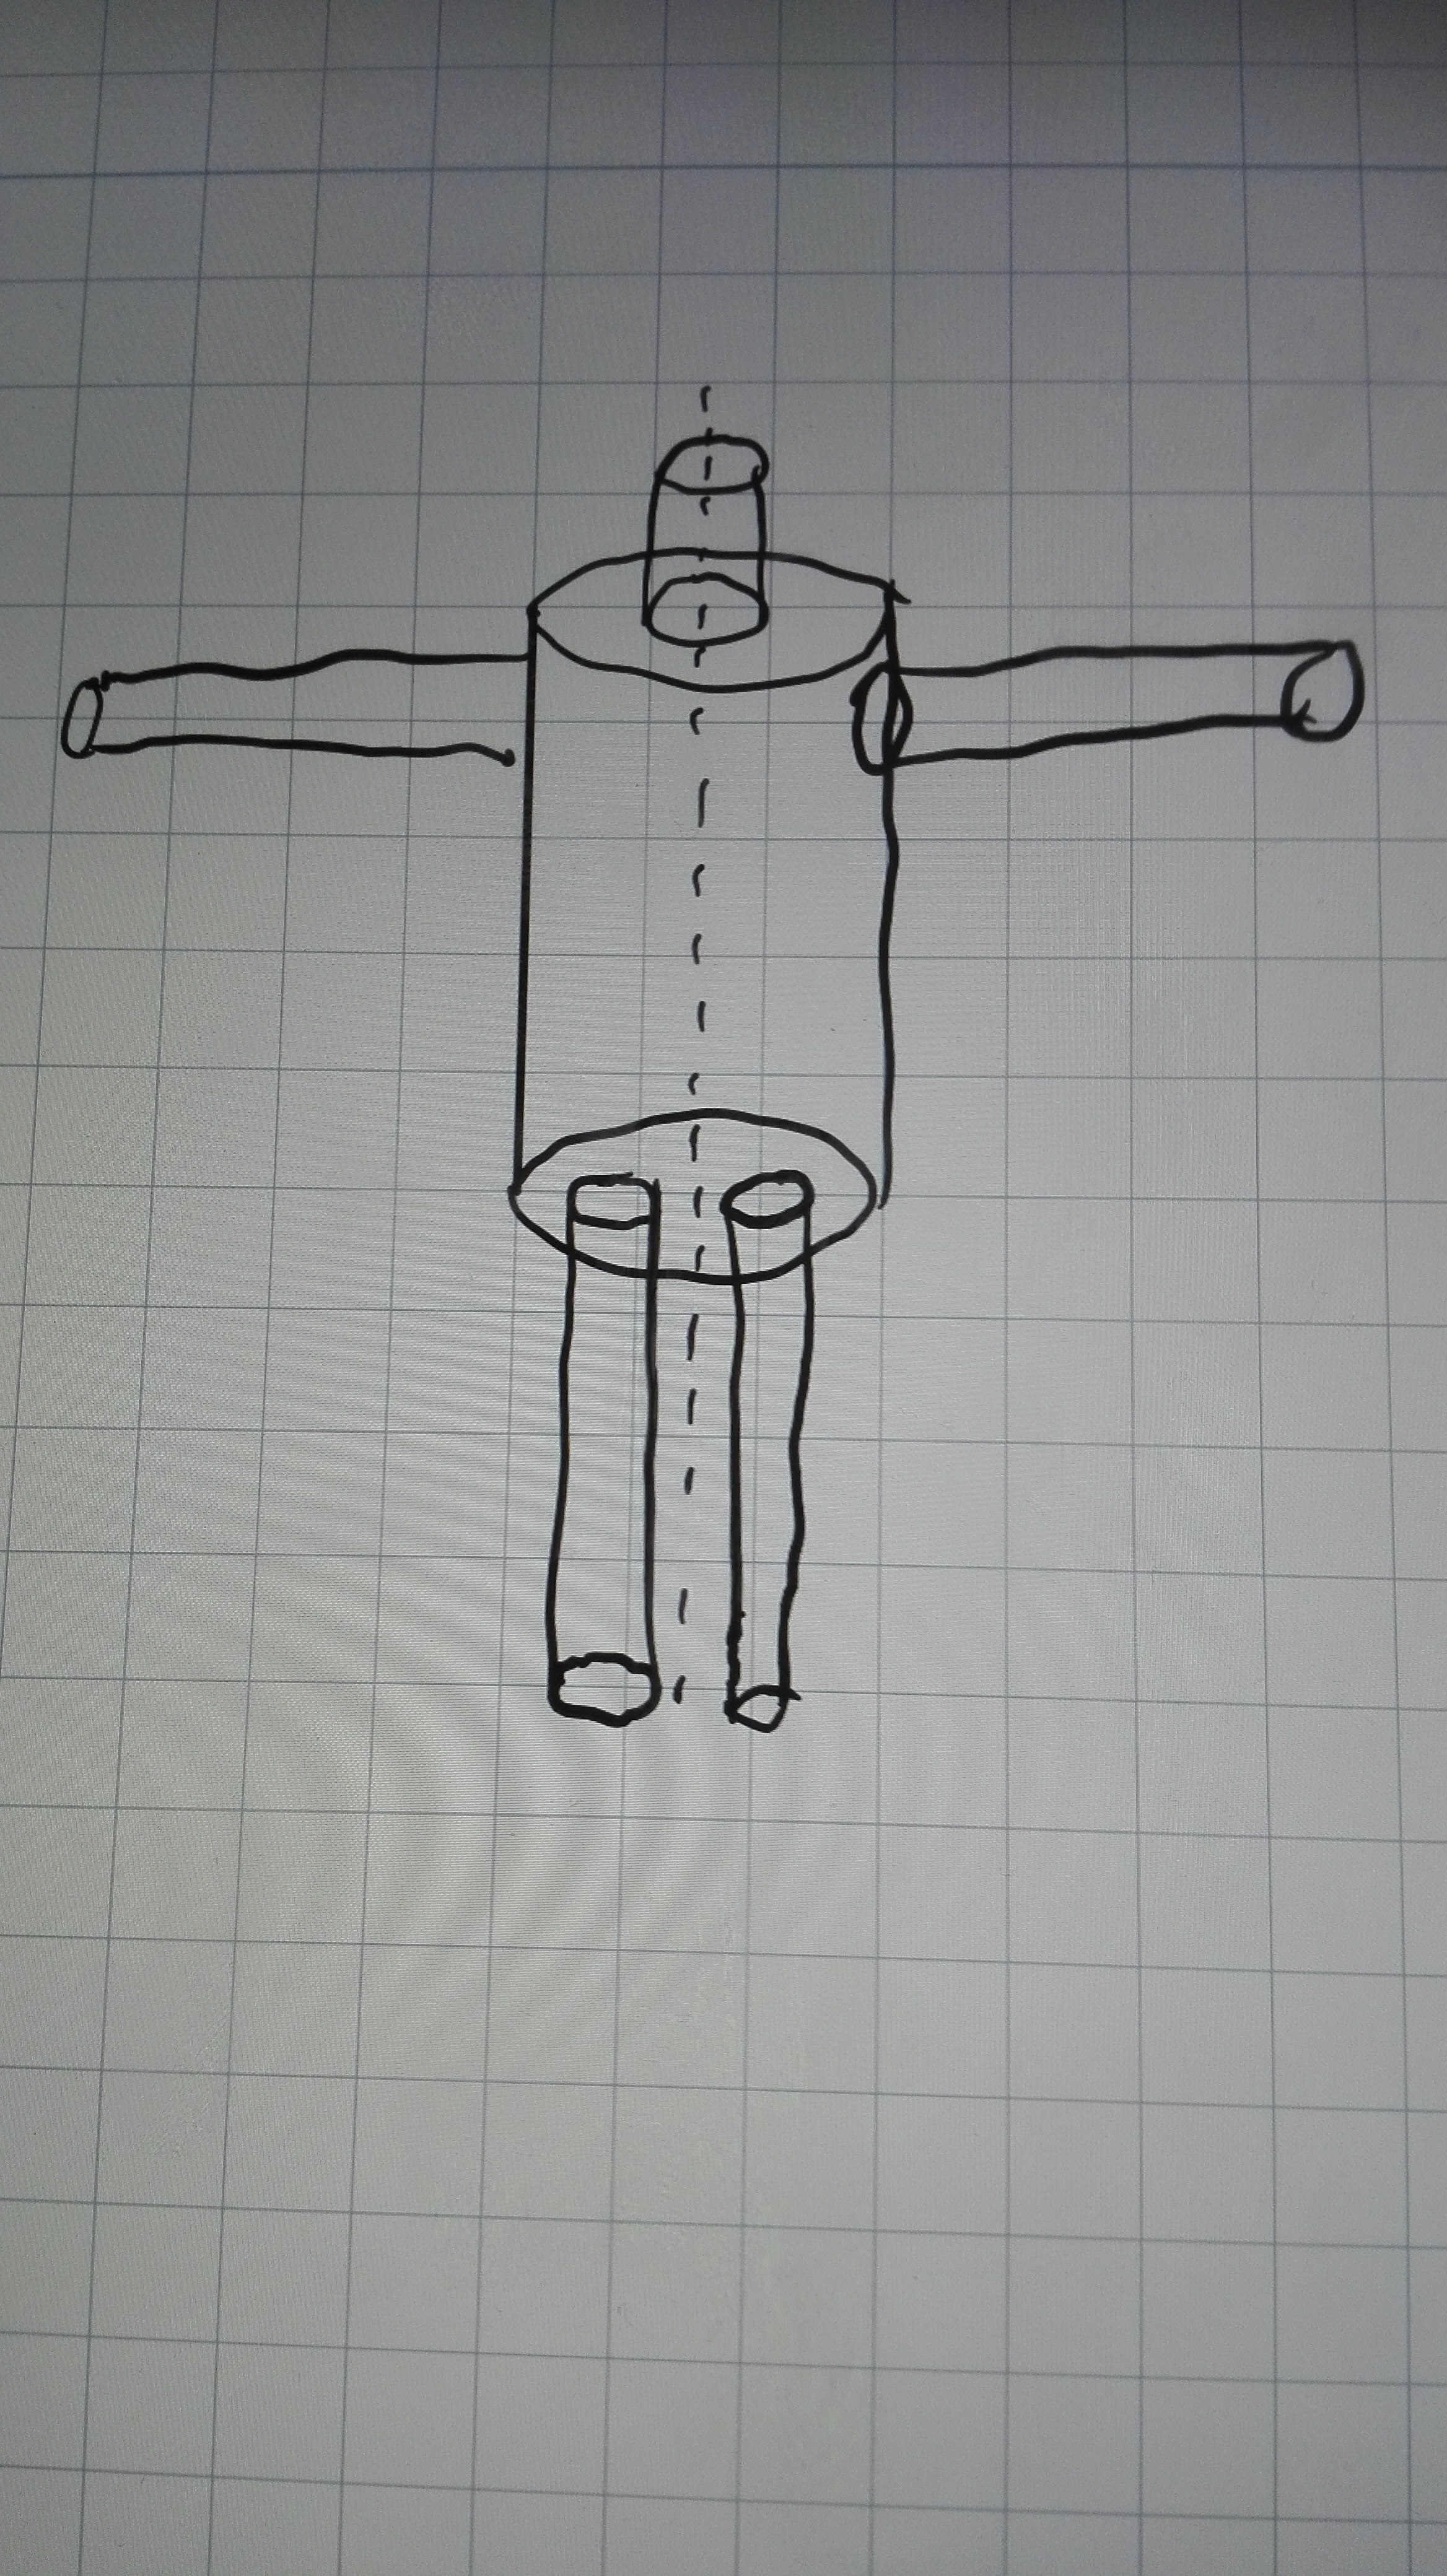
\includegraphics[width=\textwidth]{images/puppe_aus.jpg}
\caption{Puppe mit ausgestreckten Armen (Pos. 2)}
\end{subfigure}
\end{figure}

Die Massen der einzelnen Zylinder wurden mithilfer der Formel $m= \rho \cdot V$ bestimmt und lauten wie folgt:
\begin{subequations}
\begin{align}
\text{Kopf: \input{m_Kopf.tex}}\label{eq:Kopf}\\
\text{Torso: \input{m_Torso.tex}}\label{eq:Torso}\\
\text{Arm: \input{m_Arm.tex}}\label{eq:Arm}\\
\text{Bein: \input{m_Bein.tex}}\label{eq:Bein}
\end{align}
\end{subequations}

V stellt dabei die verschiedenen Zylindervolumen dar
\begin{subequations}
\begin{align}
 V_{\text{Kopf\hphantom{o}}} &= \\
 V_{\text{Torso}} &= \\
 V_{\text{Arm\hphantom{o}}} &= \\
 V_{\text{Bein\hphantom{o}}} &= ,
\end{align}
\end{subequations}
während $\rho$ die Dichte von Buchenholz wiedergibt \cite{Holzdichte}
\begin{align}
    \rho = \SI{760}{\kilo\gram\meter\tothe{-3}}
\end{align}

\flushleft{Das\;}\justifying errechnete Trägheitsmoment der Puppe in Position 1 ist:
\input{I_Puppe_an_exp_mean.tex}

\flushleft{Das\;}\justifying theoretische Trägheitsmoment der Puppe in Position 1 ist:
\input{I_Puppe_an_theo.tex}

\flushleft{Der\;}\justifying relative Fehler des Trägheitsmoments der Puppe in Position 1 ist:
\input{RF_I_Puppe_an.tex}

\subsection{Puppe (Position 2)}\justifying % Puppe 2 ---------------------------------------------------------------------------------------------------------

\flushleft{Das\;}\justifying errechnete Trägheitsmoment der Puppe in Position 2 ist:
\input{I_Puppe_aus_exp_mean.tex}

\flushleft{Das\;}\justifying theoretische Trägheitsmoment der Puppe in Position 2 ist:
\input{I_Puppe_aus_theo.tex}

\flushleft{Das\;}\justifying relative Fehler des Trägheitsmoments der Puppe in Position 2 ist:
\input{RF_I_Puppe_aus.tex}

% Diskussion %%%%%%%%%%%%%%%%%%%%%%%%%%%%%%%%%%%%%%%%%%%%%%%%%%%%%%%%%%%%%%%%%%%%%%%%%%%%%%%%%%%%%%%%%%%%%%%%%%%%%%%%%%%%%%%%%%%%%%%%%%%%%%%%%%%%%%%%%%%
\section{Diskussion}\justifying

\newpage

\printbibliography
\end{document}